\documentclass[a4paper]{article}

%Tutti gli usepackage vanno qui

\usepackage{geometry}
\usepackage[italian]{babel}
\usepackage[utf8]{inputenc}
\usepackage[T1]{fontenc}
\usepackage{tgschola}
%\usepackage{tgbonum}
\usepackage{tabularx}
\usepackage{longtable}
\usepackage{hyperref}
\usepackage{enumitem}
\usepackage[toc]{appendix}
\hypersetup{
	colorlinks=true,
	linkcolor=black,
	filecolor=magenta,      
	urlcolor=blue,
}
% Numerazione figure 
\let\counterwithout\relax
\let\counterwithin\relax
\usepackage{chngcntr}

\counterwithin{table}{subsection}
\counterwithin{figure}{subsection}

\usepackage[bottom]{footmisc}
\usepackage{fancyhdr}
\setcounter{secnumdepth}{4}
\usepackage{amsmath, amssymb}
\usepackage{array}
\usepackage{graphicx}

\usepackage{ifthen}

%\usepackage{float}
\usepackage{layouts}
\usepackage{url}
\usepackage{comment}
\usepackage{float}
\usepackage{eurosym}

\usepackage{lastpage}
\usepackage{layouts}
\usepackage{float}
\usepackage{eurosym}

%Comandi di impaginazione uguale per tutti i documenti
\pagestyle{fancy}
\lhead{
\includegraphics[scale=0.04]{../../../../latex/images/logoTWM.png}}
%Titolo del documento
\rhead{\doctitle{}}
%\rfoot{\thepage}
\cfoot{Pagina \thepage\ di \pageref{LastPage}}
\setlength{\headheight}{35pt}
\setcounter{tocdepth}{5}
\setcounter{secnumdepth}{5}
\renewcommand{\footrulewidth}{0.4pt}

% multirow per tabelle
\usepackage{multirow}

% Permette tabelle su più pagine
%\usepackage{longtable}


% colore di sfondo per le celle
\usepackage[table]{xcolor}

%COMANDI TABELLE
\newcommand{\rowcolorhead}{\rowcolor[HTML]{9b240a}} %intestazione 
% check for missing commands
\newcommand{\headertitle}[1]{\textbf{\color{white}#1}} %titolo colonna
\definecolor{pari}{HTML}{FFDBCB}
\definecolor{dispari}{HTML}{F1F7FD}

% comandi glossario
\newcommand{\glo}{$_{G}$}
\newcommand{\glosp}{$_{G}$ }


%label custom
\makeatletter
\newcommand{\uclabel}[2]{%
	\protected@write \@auxout {}{\string \newlabel {#1}{{#2}{\thepage}{#2}{#1}{}} }%
	\hypertarget{#1}{#2}
}
\makeatother

%riportare pezzi di codice
\definecolor{codegray}{gray}{0.9}
\newcommand{\code}[1]{\colorbox{codegray}{\texttt{#1}}}



% Configurazione della pagina iniziale
\newcommand{\doctitle}{Norme di Progetto}
\newcommand{\docdate}{ } % lasciare vuoto (uno carattere di spazio) per i documenti che non sono verbali, così non viene scritta la data
\newcommand{\rev}{3.0.1}
\newcommand{\stato}{Non Approvato}
\newcommand{\uso}{Interno}
\newcommand{\approv}{--De Renzis Simone}
\newcommand{\red}{Greggio Nicolò\\& Tessari Andrea}
\newcommand{\ver}{Zuccolo Giada\\& Crivellari Alberto}
\newcommand{\dest}{Three Way Milkshake\\ Prof. Vardanega Tullio\\ Prof.
 Cardin Riccardo}
\newcommand{\describedoc}{Questo documento contiene tutte le norme di progetto\textsubscript{G}, definite inizialmente o aggiunte in seguito, viene quindi aggiornato per incrementi successivi.}



 % modifica questo file
\makeindex

\usepackage{hyperref}
\usepackage{ulem}
\usepackage{listings}
\usepackage[toc,acronym]{glossaries}
\makeglossaries

\newglossaryentry{wiki}{name={wiki}, plural={wikis},%
	description={Termine di origine hawaiana che significa veloce, con cui si identifica un tipo di sito internet che permette la creazione e la modifica di pagine multimediali attraverso un'interfaccia semplice}}

\newglossaryentry{vmodel}{name={Modello a V},%
	description={Modello che illustra le relazioni tra ogni fase del ciclo di vita del software con la relativa fase di testing ad essa associata}}

\newglossaryentry{usecase}{name={caso d'uso}, plural={casi d'uso},%
	description={Un caso d'uso è un insieme di \glspl{scenario} che hanno in comune uno scopo finale (obiettivo) per un utente (\gls{attore})}}

\newglossaryentry{techbase}{name={technology baseline},%
	description={Motiva le tecnologie, i framework, e le librerie selezionate per la realizzazione del prodotto. Ne dimostra adeguatezza e fattibilità, tramite un proof of concept coerente con gli obiettivi}}

\newglossaryentry{task}{name={task}, plural={tasks},%
	description={Nel contesto del capitolato, con questo termine si identifica un compito da svolgere da parte di un unità (muletto) che consiste nel raggiungere un \acrshort{POI} e caricare o scaricare la merce}}

\newglossaryentry{stakeholder}{name={stakeholder}, plural={stakeholders},%
	description={Tutti coloro che a vario titolo hanno influenza sul prodotto e sul progetto. Sono stakeholders il committente, il proponente, gli utenti, il team di sviluppo}}

\newglossaryentry{sistematico}{name={sistematico},%
	description={Modo di lavorare metodico e rigoroso, che conosce, usa ed evolve le best practice di dominio}}

\newglossaryentry{shell}{name={shell},%
	description={Interprete dei comandi}}

\newglossaryentry{security}{name={security},%
	description={Non vulnerabilità rispetto a intrusioni}}

\newglossaryentry{scenario}{name={scenario}, plural={scenari},%
	description={Nell'ambito dello sviluppo software, sequenza di passi che descrive l'interazione tra l'\gls{attore} e il sistema, e le elaborazioni necessarie per soddisfare la richiesta dell'\gls{attore}}}

\newglossaryentry{safety}{name={safety},%
	description={Sicurezza rispetto a malfunzionamenti}}

\newglossaryentry{risorsa}{name={risorsa}, plural={risorse},%
	description={Mezzo o capacità disponibile, nello sviluppo software ad esempio le persone, il tempo, il denaro, gli strumenti necessari allo sviluppo del progetto. Le attività di progetto consumano le risorse disponibili}}

\newglossaryentry{revisione}{name={revisione}, plural={revisioni},%
	description={Esame o controllo, per lo più periodico, inteso a verificare il grado dell'efficienza, della funzionalità, della corrispondenza a determinati requisiti. Nell'ambito del corso di Ingegneria del Software, la revisione di avanzamento identifica il momento in cui il team consegna e presenta gli artefatti sviluppati durante il periodo appena trascorso}}

\newglossaryentry{requisito}{name={requisito}, plural={requisiti},%
	description={Esistono due interpretazioni principali di un requisito \begin{itemize}\item dal lato del bisogno(ovvero il cliente/utente) è la capacità necessaria a un utente per risolvere un problema o raggiungere un obiettivo\item dal lato della soluzione (ovvero lo sviluppatore) è la capacità che deve essere posseduta (o condizione che deve essere soddisfatta) da un sistema per adempiere a un obbligo \end{itemize}}}

\newglossaryentry{repository}{name={repository},%
	description={Posizione di archiviazione per pacchetti software}}

\newglossaryentry{quantificabile}{name={quantificabile},%
	description={Che permette di misurare l'efficienza e l'efficacia del suo agire}}

\newglossaryentry{proofconcept}{name={proof of concept},%
	description={Dimostratore eseguibile. Il suo codice può (ma non deve) essere usa-e-getta}}

\newglossaryentry{progetto}{name={progetto}, plural={progetti},%
	description={Insieme di attività che devono raggiungere determinati obiettivi a partire da determinate specifiche; hanno una data d'inizio e una data di fine fissate, dispongono di risorse limitate e consumano tali risorse nel loro svolgersi}}

\newglossaryentry{prodbase}{name={product baseline},%
	description={Illustra la baseline architetturale del prodotto, coerente con la \acrshort{tb}. Rappresenta il design definitivo}}

\newglossaryentry{precondizione}{name={precondizione}, plural={precondizioni},%
	description={Condizioni che devono essere soddisfatte affinché si verifichino determinati eventi successivi}}

\newglossaryentry{postcondizione}{name={postcondizione}, plural={postcondizioni},%
	description={Condizioni che devono verificarsi dopo determinati eventi}}

\newglossaryentry{planimetria}{name={planimetria}, plural={planimetrie},%
	description={Rappresentazione in piano del magazzino che ne evidenzia le caratteristiche (aree non transitabili, zone di percorrenza, punti di interesse)}}

\newglossaryentry{periodo}{name={periodo}, plural={periodi},%
	description={Nel contesto del documento, l'intervallo di tempo che intercorre tra due revisioni successive}}

\newglossaryentry{percorrenza}{name={percorrenza}, plural={percorrenze},%
	description={Nel contesto del capitolato, i vincoli relativi alle zone transitabili: \begin{itemize} \item sensi di marcia \item numero massimo di unità che vi possono transitare \end{itemize}}}

\newglossaryentry{modellosviluppo}{name={modello di sviluppo},%
	description={Principio teorico che indica il metodo da seguire nel progettare e nello scrivere un programma. Esistono tre principali modelli di sviluppo, ossia sequenziale, \gls{incrementale} ed evolutivo.}}

\newglossaryentry{milestone}{name={milestone},%
	description={Pietra miliare, istante temporale su cui si misura l'avanzamento del progetto. Viene fissata nel futuro per stabilire un avanzamento atteso. Una buona milestone è delimitata per ampiezza ed ambizioni, misurabile in termini di tempo e impegno necessario per raggiungerla, traducibile in compiti assegnabili ai membri del team e coerente con le scadenze del progetto}}

\newglossaryentry{kanban}{name={kanban},%
	description={Framework usato per implementare modelli di sviluppo Agili e DevOps. Richiede comunicazione in tempo reale tra i componenti de team e totale trasparenza. I work item vengono visualizzati su una Kanban Board, permettendo ai membri del team di vedere lo stato di ogni attività in ogni momento. Per maggiori dettagli \url{https://www.atlassian.com/agile/kanban/kanban-vs-scrum}}}

\newglossaryentry{incrementale}{name={incrementale},%
	description={Che procede per incrementi, ossia migliorie che, partendo da un impianto base, portano al raggiungimento dell'obiettivo producendo valore e limitando al massimo la regressione a stati già attraversati}}

\newglossaryentry{gitpush}{name={git-push},%
	description={Azione di git che permette di caricare le proprie modifiche locali sul server remoto condiviso del repository}}

\newglossaryentry{gitpull}{name={pull},%
	description={Comando di \gls{git} che permette di aggiornare il proprio \acrshort{repo} locale con i cambiamenti remoti}}

\newglossaryentry{git}{name={git},%
	description={Sistema di controllo del versionamento distribuito}}

\newglossaryentry{gitcommit}{name={commit}, plural={commits},%
	description={Comando di \gls{git} che permette di salvare e versionare le modifiche attuate ai file in locale}}

\newglossaryentry{gantt}{name={Gantt},%
	description={Diagramma per la pianificazione di un progetto. Esplicita le attività volte al suo svolgimento e per ognuna ne identifica data di inizio e di fine a seconda delle stime effettuate. Facilità la visualizzazione delle connessioni tra le attività e lo stato di avanzamento del progetto}}

\newglossaryentry{form}{name={form},%
	description={Interfaccia di un programma che consente a un utente di inserire e inviare uno o più dati}}

\newglossaryentry{fase}{name={fase}, plural={fasi},%
	description={Segmento temporale contiguo che che presuppone uno stazionamento in uno stato o in una transizione di ciclo di vita}}

\newglossaryentry{efficienza}{name={efficienza},%
	description={Misura dell'abilità di raggiungere l'obiettivo impiegando le risorse in maniera ottimale}}

\newglossaryentry{efficacia}{name={efficacia},%
	description={Misura della capacità di raggiungere l'obiettivo prefissato}}

\newglossaryentry{disciplinato}{name={disciplinato},%
	description={Che segue le regole che si è dato}}

\newglossaryentry{designpattern}{name={design pattern}, plural={design patterns},%
	description={Soluzione progettuale generale ad un problema ricorrente}}

\newglossaryentry{cruscotto}{name={cruscotto}, plural={cruscotti},%
	description={Interfaccia utente grafica che fornisce viste indicatori chiave di prestazione rilevanti per un particolare obiettivo o processo aziendale}}

\newglossaryentry{combobox}{name={combobox},%
	description={Controllo grafico (widget) che permette all'utente di effettuare una scelta scrivendola in una casella di testo o selezionandola da un elenco}}

\newglossaryentry{capitolato}{name={capitolato}, plural={capitolati},%
	description={Documento tecnico redatto dal cliente in cui vengono specificati i vincoli contrattuali (prezzo e scadenze) per lo sviluppo di un determinato prodotto software. Viene presentato in un bando d'appalto per trovare qualcuno che possa svolgere il lavoro richiesto}}

\newglossaryentry{bug}{name={bug},%
	description={Problema che porta al malfunzionamento del software, per esempio producendo un risultato inatteso o errato, tipicamente dovuto a un errore nella scrittura del codice sorgente di un programma}}

\newglossaryentry{bestpractice}{name={best practice}, plural={best practices},%
	description={Modo di fare noto, che abbia mostrato di garantire i migliori risultati in circostanze note e specifiche}}

\newglossaryentry{bash}{name={bash},%
	description={G:bash:bash:X:\gls{shell} Unix ed un linguaggio interpretato scritto da Brian Fox per il progetto GNU come sostituto del software gratuito per la shell Bourne}}

\newglossaryentry{baseline}{name={baseline},%
	description={Istantanea dello stato di avanzamento del progetto. Misura i risultati ottenuti e li fissa in una versione consolidata del prodotto. Può essere associata ad un rifermento temporale (\gls{milestone})}}

\newglossaryentry{attore}{name={attore}, plural={attori},%
	description={Ruolo interpretato da un utente (persona o sistema esterno) nei confronti del sistema. \begin{itemize} \item \textbf{attore primario}: attore richiede l'assistenza del sistema \item \textbf{attore secondario}: attore di cui è il sistema stesso a richiedere l'intervento \end{itemize}}}

\newglossaryentry{attivita}{name={attività},%
	description={Insieme di una o più azioni il cui completamento porta ad un avanzamento nel complesso}}

\newglossaryentry{artefatto}{name={artefatto}, plural={artefatti},%
	description={Sottoprodotto che viene realizzato durante lo sviluppo software. Sono artefatti i casi d'uso, i diagrammi delle classi, i modelli UML, il codice sorgente e la documentazione varia, che aiutano a descrivere la funzione, l'architettura e la progettazione del software}}

\newglossaryentry{agile}{name={agile},%
	description={Approccio stutturato e iterativo alla gestione dei progetti e alla sviluppo di software. Riconosce la volatilità dello sviluppo del prodotto e propone un metodo per permettere ai team di rispondere in maniera rapida a cambiamenti non pianificati e di produrre valore fin dalle prime iterazioni. Per maggiori dettagli \url{https://www.atlassian.com/agile/kanban/kanban-vs-scrum}}}

\newacronym{vcs}{VCS}{Version Control System}

\newacronym{uml}{UML}{Unified Modeling Language}

\newacronym{tb}{TB}{\gls{techbase}}

\newacronym{spa}{spa}{X}

\newacronym{rest}{REST}{REpresentational State Transfer}

\newacronym{repo}{repo}{\gls{repository}}

\newacronym{ram}{RAM}{Random Access Memory}

\newacronym{portacs}{PORTACS}{\acrshort{POI} Oriented Real Time Anti Collision System}

\newacronym{POI}{POI}{Point Of Interest}

\newacronym{poc}{PoC}{Proof of Concept}

\newacronym{pb}{PB}{\gls{prodbase}}

\newacronym{jit}{JiT}{Just in Time}

\newacronym{faas}{FaaS}{Functions as a Service}

\newacronym{eg}{e.g.}{Example given, si usa per indicare che ciò che segue è un esempio}

\newacronym{cpu}{CPU}{Central Processing Unit}

\newacronym{cms}{CMS}{Content Management System}

\newacronym{baas}{BaaS}{Backend as a Service}

\newacronym{api}{API}{Application Programming Interface}


\begin{document}
	\thispagestyle{empty}
\begin{titlepage}
	\begin{center}
		
		
\includegraphics[scale = 0.17]{../../../../latex/images/logoTWM.png}\\[0.7cm]
		

		\noindent\rule{\textwidth}{1pt} \\[0.4cm]
		\Huge \textbf{\doctitle} \\[0.1cm]
		\ifthenelse{\equal{\docdate}{ }}{ }{ \huge \textbf{\docdate} \\[0.1cm] }
		
		\noindent\rule{\textwidth}{1pt}\\[0.7cm]
		
		\large \textbf{Three Way Milkshake - Progetto "PORTACS"} \\[0.4cm] 
                \texttt{threewaymilkshake@gmail.com} \\[0.4cm]
                
		
        
        
        \large

        \begin{tabular}{r|l}
                        \textbf{Versione} & \rev{} \\
                        \textbf{Stato} & \stato{} \\
                        \textbf{Uso} & \uso{} \\                         
                        \textbf{Approvazione} & \approv{} \\                      
                        \textbf{Redazione} & \red{} \\ 
                        \textbf{Verifica} &  \ver{} \\                         
                        \textbf{Destinatari} & \parbox[t]{5cm}{ \dest{} }
                \end{tabular} 
                \\[0.3cm]
                \large \textbf{Descrizione} \\ \describedoc{} 
               

	\end{center}
\end{titlepage}
	\pagebreak

	% Registro delle modifiche
	\section*{Registro delle modifiche}

\newcommand{\changelogTable}[1]{
	
	
	\renewcommand{\arraystretch}{1.5}
	\rowcolors{2}{pari}{dispari}
	\begin{longtable}{ 
			>{\centering}p{0.07\textwidth} 
			>{}p{0.21\textwidth}
			>{\centering}p{0.17\textwidth}
			>{\centering}p{0.13\textwidth} 
			>{\centering}p{0.17\textwidth} 
			>{\centering}p{0.13\textwidth} }
		\rowcolorhead
		\headertitle{Vers.} &
		\centering \headertitle{Descrizione} &	
		\headertitle{Redazione} &
		\headertitle{Data red.} & 
		\headertitle{Verifica} &
		\headertitle{Data ver.}
		\endfirsthead	
		\endhead
		
		#1
		
	\end{longtable}
	\vspace{-2em}
	
}


\newcommand{\approvingTable}[1]{ 
	
	
	\renewcommand{\arraystretch}{1.5}
	\rowcolors{2}{pari}{dispari}
	\begin{longtable}{ 
			>{\centering}p{0.07\textwidth} 
			>{\centering}p{0.415\textwidth}
			>{\centering}p{0.13\textwidth}
			>{\centering}p{0.322\textwidth}  }
		\rowcolorhead
		\headertitle{Vers.} &
		\centering \headertitle{Descrizione} &	
		\headertitle{Data appr.} &
		\headertitle{Approvazione}
		\endfirsthead	
		\endhead
		
		#1
		
	\end{longtable}
	\vspace{-2em}
	
}
	\changelogTable{
	3.5.0 & Incremento appendice \S\ A e B & Crivellari Alberto & 2021-04-26 & -- & --
	3.4.0 & Rimossa appendice \S\ D & Crivellari Alberto & 2021-04-01 & -- & --
	\tabularnewline
	3.3.0 & Modifica sezioni \S\ 2 e \S\ 3 & Crivellari Alberto & 2021-04-01 & -- & --
	\tabularnewline
	3.2.0 & Modifica appendice \S\ B & Zuccolo Giada & 2021-03-31 & -- & --
\tabularnewline
	3.1.0 & Aggiornamento appendice \S\ C & Crivellari Alberto & 2021-03-20 & -- & --
}

\approvingTable{
    3.0.0 & Approvazione del documento & 2021-03-08 & Zuccolo Giada
}

\changelogTable{
    2.1.0 & Aggiornamento sezioni \S\ 4 e 5 & Crivellari Alberto & 2021-03-08 & Chiarello Sofia & 2021-03-08
}

\approvingTable{
    2.0.0 & Approvazione del documento & 2021-02-22 & De Renzis Simone
}

\changelogTable{
1.3.0 & Completamento stesura appendice \S\ D e \S\ B & Crivellari Alberto & 2021-02-12 & Greggio Nicolò & 2021-02-19
\tabularnewline
1.2.1 & Completamento stesura sezione \S\ 2 e \S\ 3 & Chiarello Sofia & 2021-02-11 & Tessari Andrea & 2021-02-13
\tabularnewline
1.2.0 & Stesura sezione \S\ 3 e appendice \S\ C & Chiarello Sofia & 2021-02-09 & Tessari Andrea & 2021-02-12
\tabularnewline
1.1.0 & Stesura sezione \S\ 2 & Chiarello Sofia & 2021-02-08 & Tessari Andrea & 2021-02-13
}

\approvingTable{
	1.0.0 & Approvazione del documento & 2021-01-10 & De Renzis Simone
}

\changelogTable{
0.5.1 & Aggiunta tabelle a sezione \S 4 e \S5 & Crivellari Alberto & 2021-01-08 & Greggio Nicolò & 2021-01-10
\tabularnewline
0.5.0 & Redazione sezione \S 5 & Crivellari Alberto & 2020-12-07 & Greggio Nicolò & 2021-01-10
\tabularnewline
0.4.0 & Redazione sezione \S 4 & Crivellari Alberto & 2020-12-06 & Greggio Nicolò & 2021-01-10
\tabularnewline
0.3.2 & Modifiche sezione \S 1 & Crivellari Alberto & 2020-12-30 & Greggio Nicolò & 2021-01-10
\tabularnewline
0.3.1 & Tabelle sezione \S 3 & Crivellari Alberto & 2020-12-29 & Greggio Nicolò & 2021-01-10
\tabularnewline
0.3.0 & Redazione sezione \S 3 & Tessari Andrea & 2020-12-28 & Greggio Nicolò & 2021-01-10
\tabularnewline
0.2.1 & Tabelle sezione \S 2 & Crivellari Alberto & 2020-12-20 &  Greggio Nicolò & 2021-01-09
\tabularnewline
0.2.0 & Redazione sezione \S 2 & Crivellari Alberto & 2020-12-19 & Greggio Nicolò & 2021-01-09
\tabularnewline
0.1.1 & Modifiche sezione \S 1  & Crivellari Alberto & 2020-12-18 & Greggio Nicolò & 2021-01-09
\tabularnewline
0.1.0 & Redazione sezione \S 1 & Crivellari Alberto & 2020-12-16 & Greggio Nicolò & 2021-01-09
\tabularnewline
0.0.1 & Strutturazione del documento & Tessari Andrea & 2020-12-15 & Greggio Nicolò & 2021-01-09
}


 % modifica questo file
	\end{longtable}
	\pagebreak

	% indice
	\tableofcontents
	\pagebreak

	% indice delle figure, non ci sono figure
	\listoffigures
	\pagebreak

	% indice delle tabelle
	\listoftables
	\pagebreak

	% contenuto del documento, ogni sezione in un file
	\section{Introduzione}
\subsection{Scopo del documento}
    Questo documento ha lo scopo di fissare e definire tutte le regole, convenzioni e buone pratiche utili a formare un way of working condiviso alla base da tutti i componenti del gruppo per assicurare una collaborazione efficiente ed efficace. Si discuteranno inoltre i vari strumenti che verranno adottati per facilitare lo sviluppo del progetto\textsubscript{G} e per promuovere un'organizzazione adeguata.
    Si ritiene inoltre che la definizione ed il mantenimento per incremento di un documento condiviso all'interno del gruppo di lavoro, che definisca e raccolga quanto descritto in maniera formale e centralizzata, possa favorire, in un contesto dove i membri possano variare, l'inserimento di nuovi componenti facilitandone l'ambientamento. Pur non essendo questo il contesto di lavoro attuale, è comunque una buona pratica da sperimentare e consolidare.

\subsection{Scopo del prodotto}
Il capitolato\textsubscript{G} C5 propone un progetto\textsubscript{G} in cui viene richiesto lo sviluppo di un software per il monitoraggio in tempo reale di unità che si muovono in uno spazio definito. All'interno di questo spazio, creato dall'utente per riprodurre le caratteristiche di un ambiente reale, le unità dovranno essere in grado di circolare in autonomia, o sotto il controllo dell'utente, per raggiungere dei punti di interesse posti nella mappa.  La circolazione è sottoposta a vincoli di viabilità e ad ostacoli propri della topologia dell'ambiente, deve evitare le collisioni con le altre unità e prevedere la gestione di situazioni critiche nel traffico.

\subsection{Termini, abbreviazioni ed altri documenti}
    Tutti i termini che necessitano di una spiegazione, per fornire un'adeguata comprensione, o perché possono causare ambiguità nel contesto, sono definiti nel glossario. A dispetto di tutti gli altri documenti presenti, il glossario è sotto la veste di una pagina web, più nello specifico in una wiki\textsubscript{G} di GitHub, accessibile a \href{https://github.com/Three-Way-Milkshake/docs/wiki/Glossario}{questo indirizzo}, con vocaboli suddivisi tra "Acronimi" e "Termini", disposti in ordine alfabetico al fine di facilitare la navigazione. All'interno dei documenti le voci di glossario saranno seguite da una G pedice mentre gli acronimi da una A (e.g.: voce di glossario\textsubscript{G} ; acronimo\textsubscript{A}).
    Inoltre quando si farà riferimento ad un altro documento o al documento stesso, il nome di questo sarà in maiuscoletto (e.g.: \textsc{esempio nome documento}).

\subsection{Riferimenti}
\label{ref}
    \subsubsection{Riferimenti Normativi}
        \begin{itemize}
            \item Standard ISO 12207:\\ \url{https://www.math.unipd.it/~tullio/IS-1/2009/Approfondimenti/ISO_12207-1995.pdf};
            \item Standard UML\textsubscript{A} 2.0:\\\url{https://www.omg.org/spec/UML/2.0/Superstructure/PDF};
            \item Diagrammi dei casi d'uso\textsubscript{G}:\\\url{https://www.math.unipd.it/~rcardin/swea/2021/Diagrammi\%20Use\%20Case_4x4.pdf};
            \item Diagrammi delle classi:\\\url{https://www.math.unipd.it/~rcardin/swea/2021/Diagrammi\%20delle\%20Classi_4x4.pdf};
            \item Diagrammi dei package:\\\url{https://www.math.unipd.it/~rcardin/swea/2021/Diagrammi\%20dei\%20Package_4x4.pdf};
            \item Diagrammi di attività\textsubscript{G}:\\\url{https://www.math.unipd.it/~rcardin/swea/2021/Diagrammi\%20di\%20Attivit\%c3\%a0_4x4.pdf};
            \item Diagrammi di sequenza:\\\url{https://www.math.unipd.it/~rcardin/swea/2021/Diagrammi\%20di\%20Sequenza_4x4.pdf};
            \item Standard ISO 8601:\\\url{https://www.iso.org/iso-8601-date-and-time-format.html}.
        \end{itemize}

    \subsubsection{Riferimenti Informativi}
        \begin{itemize}
        	\item \textsc{\href{https://github.com/Three-Way-Milkshake/docs/wiki/Glossario}{Glossario}}:\\per la definizione dei termini (pedice G) e degli acronimi (pedice A) evidenziati nel documento;
            \item \url{https://www.math.unipd.it/~tullio/IS-1/2020/Dispense/L03.pdf}
            \item \url{https://www.math.unipd.it/~tullio/IS-1/2020/Dispense/L06.pdf}
            \item \url{https://www.math.unipd.it/~tullio/IS-1/2020/Dispense/FC2.pdf}
            \item \url{https://www.math.unipd.it/~rcardin/swea/2021/SOLID\%20Principles\%20of\%20Object-Oriented\%20Design_4x4.pdf}
            \item \url{https://www.math.unipd.it/~tullio/IS-1/2020/Dispense/L09.pdf}
            \item \url{https://docs.github.com/en/free-pro-team@latest/actions}
            \item \url{https://www.latex-project.org/}
            \item \url{http://www.texstudio.org/}
            \item \url{https://www.xm1math.net/texmaker/}
            \item \url{https://www.atlassian.com/git/tutorials/comparing-workflows/gitflow-workflow}
            \item \url{https://github.com/about}
            \item \url{https://www.atlassian.com/software/jira}
            \item \url{https://www.atlassian.com/}
            \item \url{https://meet.google.com/}
            \item \url{https://slack.com/intl/en-it/about}
            \item \url{https://telegram.org/}
            \item \url{https://workspace.google.com/products/chat/}
        \end{itemize}

\pagebreak

	\pagebreak

	\section{Qualità del processo}

\subsection{Scopo}
Per valutare  la qualità del prodotto, il gruppo Three Way Milkshake ha deciso di avvalersi degli standard ISO/IEC 12207 e ISO/IEC 25010:2011\footnote{Vedi \hyperref[ref]{riferimenti}}, semplificandoli e riadattandoli in base alle esigenze. Le metriche per i processi individuati sono presentate di seguito, al nome si affianca una sigla che verrà utilizzata per riferirsi alle stesse successivamente.

\subsection{Processi di Sviluppo}

\subsubsection{Analisi dei Requisiti}
\paragraph{Metriche}
\begin{enumerate}
	\item []
	      \textbf{Percentuale Requisiti Obbligatori Soddisfatti (PROS)}\\
	      Indica la quantità di \glspl{requisito}\textsubscript{G} obbligatori soddisfatti rispetto al totale.
	      \begin{itemize}
		      \item \textbf{misurazione:} percentuale; $\frac{requisiti\_obbligatori\_soddisfatti}{requisiti\_obbligatori\_totali}$;
		      \item \textbf{valore preferibile:} $100\%$;
		      \item \textbf{valore accettabile:} $100\%$.
	      \end{itemize}
\end{enumerate}
\subsubsection{Progettazione}
\paragraph{Metriche}
\begin{enumerate}
	\item []
	      \textbf{Coupling Between Objects (CBO)}\\
	      Indica l'accoppiamento tra classi e oggetti; due classi si dicono accoppiate se una utilizza metodi o variabili dell'altra.
	      \begin{itemize}
		      \item \textbf{misurazione:} valore intero;
		      \item \textbf{valore preferibile:} $0\leq CBO\leq 1$;
		      \item \textbf{valore accettabile:} $0\leq CBO\leq 6$.
	      \end{itemize}
\end{enumerate}
\subsubsection{Codifica}
\paragraph{Metriche}
\begin{enumerate}
	\item[]

	      \textbf{DEPth of hierarchies(DEP)}\\
	      Indica la profondità delle gerarchie nel codice sviluppato.
	      \begin{itemize}
		      \item \textbf{misurazione:} valore intero;
		      \item \textbf{valore preferibile:} $DEP\leq2$;
		      \item \textbf{valore accettabile:} $DEP\leq3$.
	      \end{itemize}
	      \pagebreak
	\item[]
	      \textbf{LEVel of nesting (LEV)}\\
	      Indica il livello di annidamento nei vari metodi presenti nel codice prodotto.
	      \begin{itemize}
		      \item \textbf{misurazione:} valore intero;
		      \item \textbf{valore preferibile:} $1\leq LEV\leq3$;
		      \item \textbf{valore accettabile:} $\leq LEV\leq6$.
	      \end{itemize}
	\item[]
	      \textbf{PARametri per metodo (PAR)}\\
	      Indica il numero di parametri presenti nei metodi sviluppati nel codice.
	      \begin{itemize}
		      \item \textbf{misurazione:} valore intero;
		      \item \textbf{valore preferibile:} $PAR\leq 4$;
		      \item \textbf{valore accettabile:} $PAR\leq 6$.
	      \end{itemize}
	\item[]
	      \textbf{Rapporto Codice Commenti (RCC)}\\
	      Indica il rapporto tra le linee di codice e le linee di commento all'interno del file.
	      \begin{itemize}
		      \item \textbf{misurazione:} valore decimale; $\frac{linee\_codice}{linee\_commento}$;
		      \item \textbf{valore preferibile:} $RCC\geq 0.4$;
		      \item \textbf{valore accettabile:} $RCC\geq 0.2$.
	      \end{itemize}
\end{enumerate}

\subsection{Processi di Supporto}
\subsubsection{Pianificazione}
\paragraph{Metriche}
\begin{enumerate}
	\item[]
	      \textbf{Budget At Completion (BAC)}\\
	      Indica il budget totale allocato per il \gls{progetto}\textsubscript{G}
	      \begin{itemize}
		      \item \textbf{misurazione:} valore intero;
		      \item \textbf{valore preferibile:} $preventivo$;
		      \item \textbf{valore accettabile:} $preventivo-5\%\leq BAC\leq preventivo+5\%$.
	      \end{itemize}
	\item[]
	      \textbf{Earned Value (EV)}\\
	      Indica la quantità di guadagno ottenuta dal lavoro effettuato fino al momento del calcolo.
	      \begin{itemize}
		      \item \textbf{misurazione:} $preventivo\cdot \%\_lavoro\_pianificato$;
		      \item \textbf{valore preferibile:} $EV\geq 0$;
		      \item \textbf{valore accettabile:} $EV\geq 0$.
	      \end{itemize}
	\item[]
	      \textbf{Planned Value (PV)}\\
	      Indica la quantità di guadagno stimata sul lavoro pianificato al momento del calcolo.
	      \begin{itemize}
		      \item \textbf{misurazione:} $preventivo \cdot \%\_lavoro\_pianificato$;
		      \item \textbf{valore preferibile:} $PV\geq 0$;
		      \item \textbf{valore accettabile:} $PV\geq 0$;
	      \end{itemize}
	\item[]
	      \textbf{Schedule Variance (SV)}\\
	      Indica l'anticipo o il ritardo del lavoro effettuato rispetto alla pianificazione.
	      \begin{itemize}
		      \item \textbf{misurazione:} $EV-PV$;
		      \item \textbf{valore preferibile:} $SV\geq 0$;
		      \item \textbf{valore accettabile:} $SV=0$.
	      \end{itemize}
	\item[]
	      \textbf{Actual Cost (AC)}\\
	      I costi sostenuti fino al momento del calcolo.
	      \begin{itemize}
		      \item \textbf{misurazione:} valore intero;
		      \item \textbf{valore preferibile:} $0\leq AC\leq PV$;
		      \item \textbf{valore accettabile:} $0\leq AC\leq budget$.
	      \end{itemize}
	\item[]
	      \textbf{Cost Variance (CV)}\\
	      La differenza tra il costo del lavoro ad ora effettuato ed quello preventivato.
	      \begin{itemize}
		      \item \textbf{misurazione:} $EV-AC$;
		      \item \textbf{valore preferibile:} $CV\geq 0$;
		      \item \textbf{valore accettabile:} $CV\geq 0$.
	      \end{itemize}
\end{enumerate}
\subsubsection{Verifica}
\paragraph{Metriche}
\begin{enumerate}
	\item[]
	      \textbf{Code Coverage (CC)}\\
	      Indica la quantità di codice che viene effettivamente eseguito durante i test; aiuta a valutare la completezza di questi.
	      \begin{itemize}
		      \item \textbf{misurazione:} percentuale; $\frac{linee\_codice\_verificate}{linee\_codice\_totali}$;
		      \item \textbf{valore preferibile:} $100\%$;
		      \item \textbf{valore accettabile:} $75\%$.
	      \end{itemize}
\end{enumerate}
\subsubsection{Documentazione}
\paragraph{Metriche}
\begin{enumerate}
	\item[]
	      \textbf{Indice di Gulpease(IG)}\\
	      Indica la leggibilità di un testo, tarato sulla lingua italiana.
	      \begin{itemize}
		      \item \textbf{misurazione:} [ $89+ \frac{300\cdot (num\_frasi) - 10\cdot (num\_lettere)}{num\_parole}$ ];
		      \item \textbf{valore preferibile:} $80\leq IG\leq 100$;
		      \item \textbf{valore accettabile:} $50\leq IG\leq 100$.
	      \end{itemize}
\end{enumerate}
\pagebreak
\subsubsection{Tabella riassuntiva}
%tabella
\begin{table}[H]
	\begin{center}
		\caption{Tabella riassuntiva metriche di processo}
		\begin{tabular}{cc!{\color[HTML]{9b240a}\vrule width 0.05cm}cc}
			\rowcolorhead
			\headertitle{Codice} & \headertitle{Tipo Processo} & \headertitle{Valori Preferibili} & \headertitle{Valori Accettabili} \\

			$PROS$               & Analisi dei Requisiti       & $100\%$                          & $100\% $                           \\
			$CBO$                & Progettazione               & $0\leq CBO\leq 1$                & $0 \leq CBO \leq 6$                    \\
			$DEP$                & Codifica                    & $DEP\leq 2$                      & $DEP \leq 3     $                    \\
			$LEV$                & Codifica                    & $1\leq LEV \leq 3$               & $1\leq LEV \leq 6$                    \\
			$PAR$                & Codifica                    & $PAR\leq 4$                      & $PAR\leq6     $                    \\
			$RCC$                & Codifica                    & $RCC \geq 0.4$                   & $RCC\geq0.2   $                    \\
			$BAC$                & Pianificazione              & $preventivo$                     & $preventivo \pm 5\%$      \\
			$EV$                 & Pianificazione              & $EV \geq 0$                      & $EV\geq0$                          \\
			$PV$                 & Pianificazione              & $PV \geq0$                       & $PV\geq0$                          \\
			$SV$                 & Pianificazione              & $SV \geq 0$                      & $SV=0   $                          \\
			$AC$                 & Pianificazione              & $0 \leq AC \leq PV$              & $0 \leq AC\leq budget$       \\
			$CV$                 & Pianificazione              & $CV \geq 0 $                     & $CV\geq 0$                          \\
			$CC$                 & Verifica                    & $100\% $                         & $75\%    $                         \\
			$IG$                 & Documentazione              & $80\leq IG \leq 100$             & $50\leq IG \leq 100$                  \\
		\end{tabular}

	\end{center}
\end{table}
	\pagebreak

	\section{Qualità del prodotto}
Per valutare  la qualità del prodotto, il gruppo Three Way Milkshake ha deciso di avvalersi dello standard ISO/IEC$_G$ 9126.\\
Questo modello è mirato a  migliorare l'organizzazione e i processi di una società software.\\
Di seguito verrà descritto il modello della qualità del software, in:
\begin{itemize}
	\item Funzionalità
	\item Affidabilità
	\item Efficienza
	\item Usabilità
	\item Manutenibilità
	\item Portabilità
\end{itemize}

\subsection{Funzionalità}
La funzionalità è la capacità di un prodotto di rispondere ad esigenze specifiche.\\
In questo caso le esigenze vengono descritte nel documento Analisi dei Requisiti.
\subsubsection{Obiettivi}
\begin{itemize}
	\item Appropriatezza: Capacità del software di riuscire a svolgere tutte le funzionalità prefissate con l'utente;
	\item Accuratezza: Capacità del software di svolgere correttamente ciò che era stato precedentemente concordato;
	\item Interoperabilità: Capacità del software di operare con più sistemi;
	\item Conformità: Capacità del software di aderire agli standard relativi alla funzionalità;
	\item Sicurezza: Capacità del software di non permettere alle persone non autorizzate di accedere o modificare dati sensibili dell'utente; consente alle persone autorizzate di accedere ai dati.
\end{itemize}

\subsubsection{Metriche}
Viene specificata la completezza del software attraverso la seguente formula:
\begin{center}
	$C = (1-($Funzionalità non implementate$ / $Funzionalità implementate$))$
\end{center}
Con i valori:\\
preferibile = 1;\\
accettabile = 1.

\subsection{Affidabilità}
L'affidabilità è la capacità di un certo software di mantenere un certo livello di prestazioni in determinate condizioni in un certo periodo.
\subsubsection{Obiettivi}
\begin{itemize}
	\item Maturità: Capacità del prodotto di dare risultati corretti, esenti da malfunzionamenti o errori;
	\item Tolleranza agli errori: Capacità del prodotto di poter essere usabile anche in presenza di malfunzionamenti o casi derivanti un uso scorretto del software;
	\item Recuperabilità: Capacità del prodotto di recuperare almeno le informazioni rilevanti in seguito ad un malfunzionamento;
	\item Aderenza: Capacità del prodotto di aderire a standard inerenti all'affidabilità.
\end{itemize}
\subsubsection{Metriche}
Viene specificata l'abilità del software di resistere a malfunzionamenti attraverso la seguente formula:
\begin{center}
	$R = $Numero di errori$ / $Numero di test eseguiti
\end{center}
Con i valori:\\
preferibile = 0;\\
accettabile < 0.15.

\subsection{Efficienza}
L'efficienza è la capacità del software di poter offrire un determinato livello di prestazioni in date condizioni in un certo periodo.
\subsubsection{Obiettivi}
\begin{itemize}
	\item Comportamento rispetto al tempo: Capacità del prodotto di fornire adeguati livelli di elaborazione, velocità e tempi di risposta;
	\item Utilizzo delle risorse: Capacità del prodotto di utilizzare le risorse in maniera adeguata;
	\item Conformità: Capacità del prodotto di aderire a standard sull'efficienza.
\end{itemize}
\subsubsection{Metriche}
Visto che il proponente non ha incluso dettagli relativi alla qualità dell'efficienza, non verranno proposte metriche per questa sezione.

\subsection{Usabilità}
L'usabilità è la capacità del prodotto di essere compreso ed utilizzato dall'utente senza difficoltà tenendo conto certe condizioni.

\subsubsection{Obiettivi}
\begin{itemize}
	\item Comprensibilità: Capacità del prodotto di visualizzare le varie funzionalità del software e permette all'utente di capire se il software è indicato per le sue esigenze;
	\item Apprendibilità: Capacità del prodotto di aumentare nel tempo l'abilità dell'utente di sfruttare il software;
	\item Operabilità: Capacità del prodotto che permette agli utenti di farne uso per i loro scopi;
	\item Attrattiva: Capacità del prodotto di rendere più piacevolo l'utilizzo del software;
	\item Conformità: Capacità del prodotto di aderire a standard relativi all'usabilità.
\end{itemize}

\subsubsection{Metriche}
Viene specificata la facilità con cui l'utente riesce a raggiungere ciò che vuole attraverso il conteggio del numero di tocchi o click necessari al suo raggiungimento.\\
Si considera la capacità dell'operatore di visualizzare la propria lista delle task:\\
Numero di tocchi o click preferibili < 4;\\
accettabile < 6. \\ \space \\
Viene specificata la facilità con cui l'utente riesce a raggiungere ciò che vuole attraverso il conteggio dei secondi necessari al suo raggiungimento.\\
Si considera la capacità dell'operatore di visualizzare la propria lista delle task:\\
valore dei secondi preferibile < 15;\\
accettabile < 40. \\ \space \\
Viene specificata la profondità gerarchica massima dei collegamenti e delle funzionalità presenti all'interno del software:\\
valore preferibile < 4;\\
accettabile < 6.

\subsection{Manutenibilità}
Capacità del prodotto di essere modificato anche in futuro.
\subsubsection{Obiettivi}
\begin{itemize}
	\item Analizzabilità: Facilità con cui è possibile interpretare il codice del software;
	\item Modificabilità: Capacità per cui risulta non troppo oneroso modificare il codice del software;
	\item Stabilità: Capacità del software di evitare errori inaspettati derivanti da modifiche errate;
	\item Testabilità: Capacità del prodotto di essere testato al fine di validare le modifiche al codice sorgente.
\end{itemize}
\subsubsection{Metriche}
Viene specificata la leggibilità del software attraverso la seguente formula:
\begin{center}
	$L = $Numero di linee di codice commentate$ / $Numero di linee di codice
\end{center}
Con i valori:\\
preferibile > 0.15;\\
accettabile > 0.10.

\subsection{Portabilità}
La portabilità è la capacità del software di poter funzionare senza tener conto di uno specifico ambiente di lavoro.
\subsubsection{Obiettivi}
\begin{itemize}
	\item Adattabilità: Capacità del prodotto di essere adattato per diversi ambienti operativi;
	\item Installabilità: Capacità del prodotto di essere installato in uno specificato ambiente operativo;
	\item Conformità: Capacità del software di aderire a standard relativi alla portabilità;
	\item Sostituibilità: Capacità del software di sostituire un altro prodotto con le stesse funzionalità.
\end{itemize}
\subsubsection{Metriche}
IL software dovrà eseguire solamente su ambiente Docker, quindi non sono necessarie varie metriche.
\subsection{Tabella Riassuntiva}
%tabella
\begin{table}[H]
	\begin{center}
		\caption{Tabella riassuntiva metriche di processo}
		\begin{tabular}{p{0.25\linewidth} p{0.25\linewidth}c!{\color[HTML]{9b240a}\vrule width 0.05cm}cc}
			\rowcolorhead
			\headertitle{Nome Metrica} & \headertitle{Descrizione} & \headertitle{Tipo Capacità} & \headertitle{Val. Pref.} & \headertitle{Val. Accett.}\\
			
			Completezza del Software Cs & Funzionalità non implementate rispetto alle funzionalità implementate & Funzionalità & Cs = 1 & Cs = 1\\
			Affidabilità del Software A & Errori rispetto al numero di test eseguiti & Affidabilità & A = 0 & A < 0.15\\
			Numero di tocchi/click necessari C & Numero di tocchi o click necessari per visualizzare la propria lista di task & Usabilità & C < 4 & C < 6\\
			Numero di secondi necessari S & Numero di secondi necessari per visualizzare la propria lista di task & Usabilità & S < 15 & S < 40\\
			Profondità gerarchica P & Profondità gerarchica massima dei collegamenti e funzionalità presenti all'interno del software & Usabilità & P < 4 & P < 6\\
			Leggibilità software L & Numero di linee di codice commentate rispetto al totale di linee di codice & Manutenibilità & L > 0.15 & L > 0.10\\
			
			
		\end{tabular}
		
	\end{center}
\end{table}

	\pagebreak

	\section{Test}

\subsection{Specifica dei test}

Per garantire la qualità del prodotto, \textit{Three Way Milkshake} adotta il Modello a V per verificare tramite test ogni passo della produzione software.\\Qui vedremo un immagine rappresentativa del \gls{vmodel}\textsubscript{G} (o V-Model), quest'ultimo si puo' schematizzare posizionando il tempo nell'asse delle ascisse e il livello di astrazione nell'asse delle ordinate.\\Il modello idealmente si divide in 2 rami.\\Il ramo sinistro contiene le fasi di progettazione e ideazione; il ramo destro contiene le fasi di testing e integrazione.
\begin{figure}[h!]
	\centering
	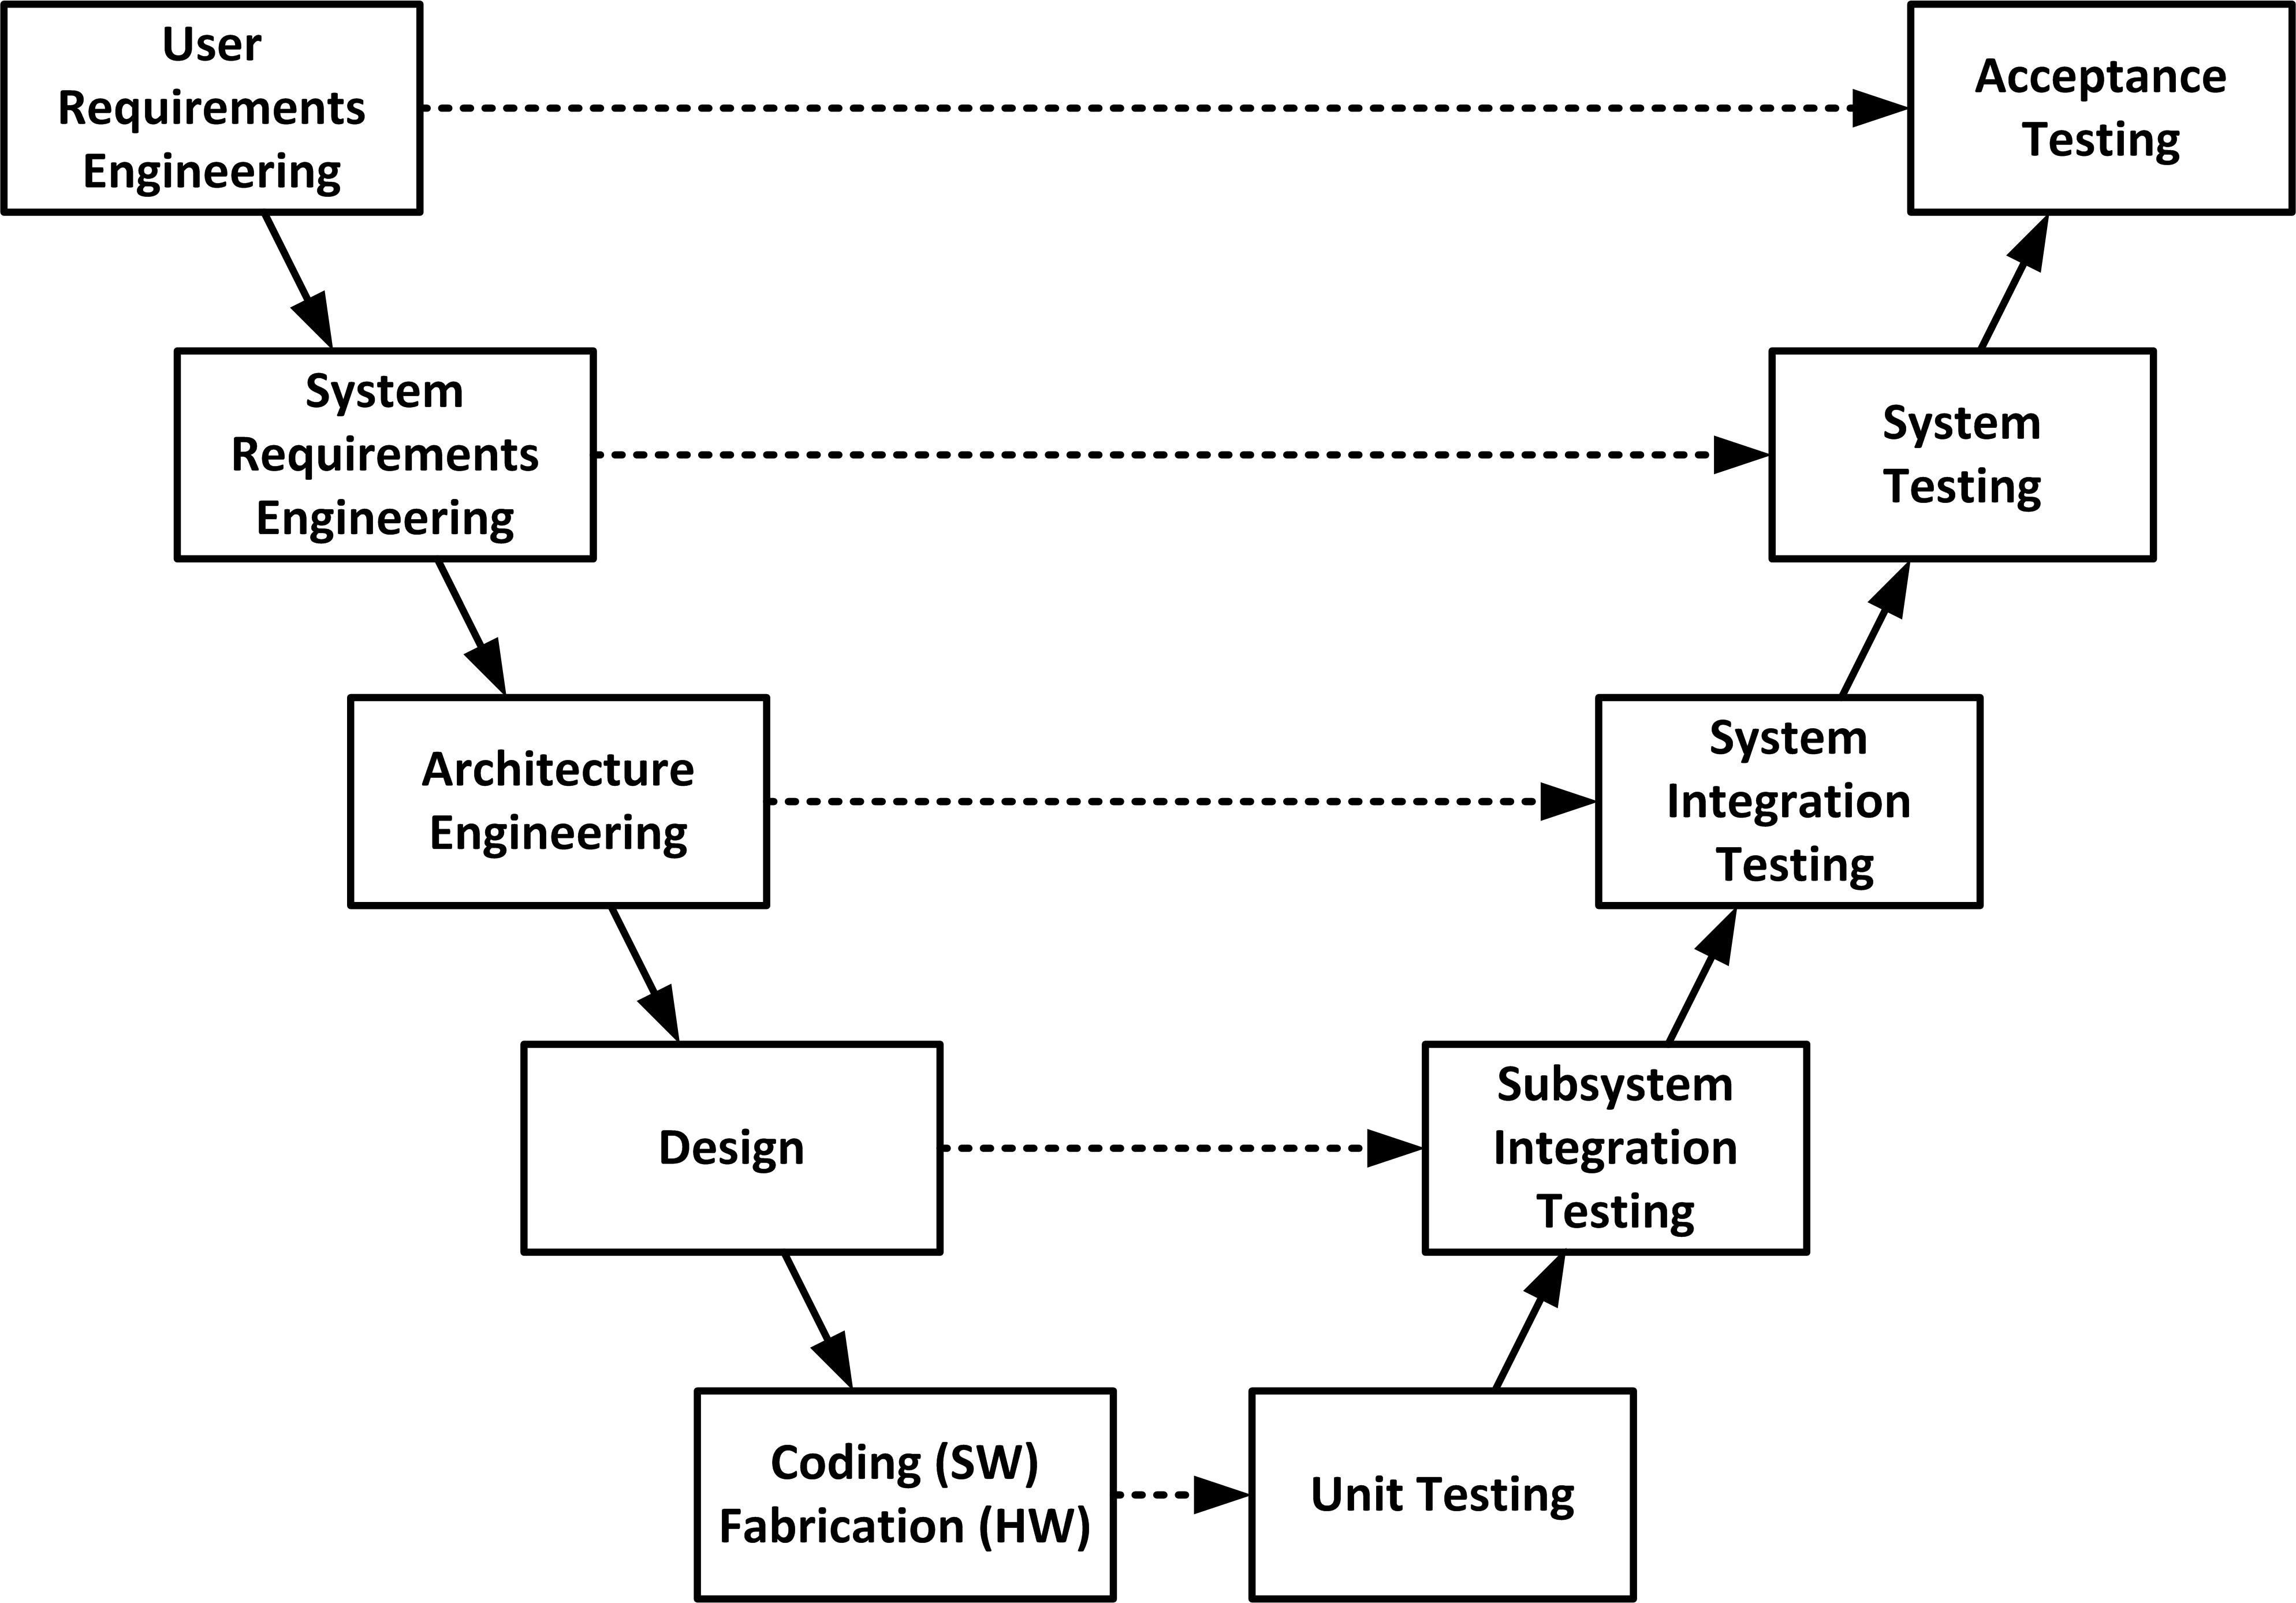
\includegraphics[scale=0.6]{res/images/v_model.jpg}
	\caption{Figura esplicativa del \gls{vmodel}\textsubscript{G}}
\end{figure}

\subsection{Test di accettazione}

\subsection{Test di sistema}

\subsection{Test di integrazione}

\subsection{Test d'unità}

\subsection{Resoconto attività di verifica}
\subsubsection{Esiti dell'indice di Gulpease}

	\pagebreak

	\section{Resoconto \gls{attivita}\textsubscript{G} di verifica}
\subsection{Esiti dell'indice di Gulpease}
% COMPILARE VALORI GULPEASE e METTERE DATE VERBALI
\begin{table}[H]
	\begin{center}
		\caption{Tabella dei valori Gulpease}
		\begin{tabular}{ccc}
			\rowcolorhead
			\headertitle{Nome Documento} & \headertitle{Valore Gulpease} & \headertitle{Esito}\\

			\textsc{Analisi dei Requisiti} v1.0.0 & & Superato\\
			\textsc{Glossario} v1.0.0 & & Superato\\
			\textsc{Norme di Progetto} v1.0.0 & & Superato\\
			\textsc{Piano di Qualifica} v1.0.0 & & Superato\\
			\textsc{Piano di Progetto} v1.0.0 & & Superato\\
			\textsc{Verbale Esterno 1} & & Superato\\
			\textsc{Verbale Esterno 2} & & Superato\\
			\textsc{Verbale Interno 1} & & Superato\\
			\textsc{Verbale Interno 2} & & Superato\\
			\textsc{Verbale Interno 3} & & Superato\\
			\textsc{Verbale Interno 4} & & Superato\\
			\textsc{Verbale Interno 2021-01-04} & & Superato\\

		\end{tabular}

	\end{center}
\end{table}

	\pagebreak
	\printglossary[type=\acronymtype,title=Lista degli Acronimi]
	\printglossary[title=Glossario dei Termini]
\end{document}
